\documentclass[12pt]{article}
\usepackage{amsmath}
\usepackage{graphicx}
\begin{document}
\title{Computer Science 143, Homework 1}
\date{April 18th, 2018}
\author{Michael Wu\\UID: 404751542}
\maketitle

\section*{Part 1}

\paragraph{a)}

\begin{verbatim}
CREATE TABLE scooter (
  id INT PRIMARY KEY NOT NULL,
  online BOOLEAN NOT NULL,
  homeLocation VARCHAR(100) NOT NULL
);

CREATE TABLE user (
  id INT PRIMARY KEY NOT NULL,
  creditCard CHAR(16),
  expiration DATE,
  email VARCHAR(100) NOT NULL
);
\end{verbatim}

\paragraph{b)}

\begin{verbatim}
CREATE TABLE trip (
  id INT PRIMARY KEY NOT NULL,
  uid INT NOT NULL,
  sid INT NOT NULL,
  startLatitude DOUBLE NOT NULL,
  startLongitude DOUBLE NOT NULL,
  endLatitude DOUBLE NOT NULL,
  endLongitude DOUBLE NOT NULL,
  startTime DATETIME NOT NULL,
  endTime DATETIME NOT NULL,
  price DECIMAL(20,2) NOT NULL,
  FOREIGN KEY uid REFERENCES user(id),
  FOREIGN KEY sid REFERENCES scooter(id)
);
\end{verbatim}
The attributes \texttt{uid} and \texttt{sid} are foreign keys.

\paragraph{c)}

The first way of inserting at the beginning of a trip and updating later has the advantage
that a record of the trip is created as soon as the trip begins. So even if a phone fails
to communicate with the server anymore, the company will know that a trip occurred and
could possibly charge the user a fee. However it will require changing the database, which
means it could require increased processing power. The second way of inserting at the end of the trip
has the advantage that no updates will be necessary in the database, reducing the amount of
work that the database has to do. However, since trip information is cached, if a phone crashes
trip information may be lost. I would prefer the first way so that we can keep track of partial
information and avoid losing data. An alternative solution would be to create a \texttt{startTrip}
table and an \texttt{endTrip} table that contain the relative information generated at the start
and end of the trip. This would make it so that trip information could be split up in a more intuitive
way.

\pagebreak

\paragraph{d)}

The table schema is shown below.
\begin{figure}[h]
    \begin{center}
        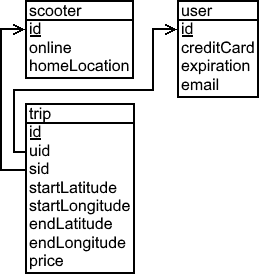
\includegraphics[width=2.5in]{problem1d.png}
    \end{center}
\end{figure}

\section*{Part 2}

\paragraph{a)}

\begin{verbatim}
SELECT HOUR(DateTime), SUM(Throughput)
FROM rides2017
GROUP BY HOUR(DateTime);
\end{verbatim}

\paragraph{b)}

\begin{verbatim}
SELECT Origin, Destination
FROM rides2017
WHERE DAYOFWEEK(DateTime)>1 AND DAYOFWEEK(DateTime)<7
GROUP BY Origin, Destination
ORDER BY SUM(Throughput) DESC
LIMIT 1;
\end{verbatim}

\filbreak

\paragraph{c)}

\begin{verbatim}
SELECT Destination, AVG(Throughput) AS Average
FROM
  (SELECT Destination, SUM(Throughput) AS Throughput
  FROM rides2017
  WHERE DAYOFWEEK(DateTime)=2
    AND HOUR(DateTime)>=7
    AND HOUR (DateTime)<10
  GROUP BY Destination, DATE(DateTime))
  AS mondayRushHourThroughput
GROUP BY Destination
ORDER BY Average DESC
LIMIT 5;
\end{verbatim}

\paragraph{d)}

\begin{verbatim}
SELECT Origin
FROM
  (SELECT Origin, SUM(Throughput) AS Throughput
  FROM rides2017
  GROUP BY Origin, DateTime) AS hourlyThroughput
GROUP BY Origin
HAVING MAX(Throughput)>100*AVG(Throughput);
\end{verbatim}

\paragraph{e)}

\[
        \pi_{\text{hour}, \text{trips}/100}(
                \sigma_{(\text{hour}>=7 \wedge \text{hour}<10)\vee (\text{hour}>=17 \wedge \text{hour}<19)}(
                        \text{hourly\_ridership}))
\]

\paragraph{f)}

\begin{multline*}
        \pi_{\text{Station},\text{DateTime},\text{Riders},\text{Condition}}(\\
                \sigma_{\text{Condition}=\text{sunny}\vee\text{Condition}=\text{rainy}}(\\
                        \text{Occupancy} \bowtie \text{Weather}))
\end{multline*}

\end{document}